% Copyright © 2013, 2014 Lénaïc Bagnères, hnc@singularity.fr

% Licensed under the Apache License, Version 2.0 (the "License");
% you may not use this file except in compliance with the License.
% You may obtain a copy of the License at
%
% http://www.apache.org/licenses/LICENSE-2.0
%
% Unless required by applicable law or agreed to in writing, software
% distributed under the License is distributed on an "AS IS" BASIS,
% WITHOUT WARRANTIES OR CONDITIONS OF ANY KIND, either express or implied.
% See the License for the specific language governing permissions and
% limitations under the License.


\documentclass[a4paper]{article}

\usepackage[utf8]{inputenc}
\usepackage[T1]{fontenc}
\usepackage[francais]{babel}
\usepackage[bookmarks=true,colorlinks,linkcolor=blue]{hyperref}

\usepackage[top=3cm,bottom=2cm,left=2.5cm,right=2.5cm]{geometry}

\usepackage{verbatim}

\usepackage{graphicx}
\usepackage{wrapfig}
\usepackage{subfig}

\usepackage{url}

\usepackage{listings}
\lstset{
	  breaklines = true
	, language = C++
	, numbers = left
	, tabsize = 4
	, basicstyle = \small\ttfamily
	, keywordstyle = \color{blue}
	, commentstyle = \color{green}
	, stringstyle = \color{red}
	, identifierstyle = \ttfamily
	, columns = flexible
}


\hypersetup{
  pdftitle={Rapport},
  pdfsubject={},
  pdfkeywords={},
  pdfauthor={Prénom \textsc{Nom}}
}

\title{Rapport}
\author{Prénom \textsc{Nom}}
%\date{}


\begin{document}

	\maketitle

	\tableofcontents

	\section*{Introduction}

		Les différents textes proviennent d'articles de Wikipédia; \url{http://fr.wikipedia.org/wiki/LaTeX} pour l'introduction. \\
		
		\LaTeX{} est un langage et un système de composition de documents créé par Leslie \textsc{Lamport} en 1983. Plus exactement, il s'agit d'une collection de macro-commandes destinées à faciliter l'utilisation du «processeur de texte» TeX de Donald \textsc{Knuth}. \\

		Du fait de sa relative simplicité, il est devenu la méthode privilégiée d'écriture de documents scientifiques employant TeX. Il est particulièrement utilisé dans les domaines techniques et scientifiques pour la production de documents de taille moyenne ou importante (thèse ou livre, par exemple). Néanmoins, il peut être aussi employé pour générer des documents de types variés (par exemple, des lettres, ou des transparents\footnote{Ou des rendus de TP ;)}).
		

	\section{Utilisation basique}

		\subsection{Texte \& listes}

			Vous pouvez mettre des mots en \emph{importance} avec \verb$\emph{mot}$, en \textbf{gras} avec \verb$\textbf{mot}$, en \texttt{lettres d'imprimerie} avec \verb$\texttt{mot}$ et en \textsc{petites capitales} avec \verb$\textsc{mot}$. \\

			Le retour à la ligne se fait avec \verb$\\$. Pour commencer un nouveau paragraphe, il faut sauter une ligne. Ne mettez pas d'espace entre les mots et les signes de ponctuation, \LaTeX{} le fait correctement pour vous. Un espace insécable peut être insérer avec le caractère \verb$~$. \\
			
			Liste avec puces:
			\begin{itemize}
				\item Un premier élément
				\item Un deuxième élément
				\item ...
			\end{itemize} ~

			Liste avec compteur automatique:
			\begin{enumerate}
				\item Un
				\item Deux
				\item ...
			\end{enumerate} ~

			Liste personnalisée:
			\begin{enumerate}
				\item[a] Un premier élément
				\item[z] Un deuxième élément
				\item[e] ...
			\end{enumerate} ~

		\subsection{Formule mathématique}

			Exemple d'une formule mathématique $1 + 9 = 10$ dans le texte. \\
			
			Exemple d'une formule mathématique seule sur sa ligne \[ \sum_{n=1}^{+\infty} \frac{1}{n^2} = \frac{\pi^2}{6} \]


	\section{Autres utilisations}

		\subsection{Figure}

			L'environnement figure permet de placer des flottants. Un titre peut être mis au dessus ou en dessus. \LaTeX{} gère lui-même l'espace. Des options peut être passé pour forcer le placement des figures (\verb$\begin{figure}[h]$ par exemple) même si cela est à éviter.

			\begin{figure}[h]
			\caption{Exemple de figure}
			\centering Contenu de la figure
			\end{figure}

		\subsection{Images}

			Avec \texttt{pdflatex} vous pouvez inclure des images matricielles (jpeg, png, ...) et vectorielles (pdf, eps, ...). \\
			
			\begin{figure}[h]
			\centering 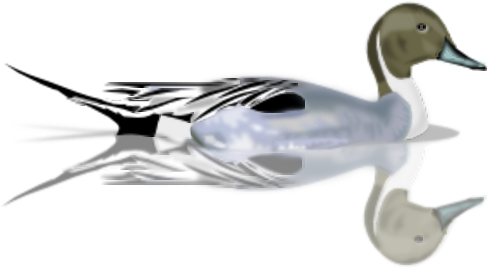
\includegraphics[width=0.5\textwidth]{img/Canard_Pilet.pdf}
			\caption{Un canard pilet vectoriel}
			\end{figure}

		\subsection{Images incrustées}

			\noindent Texte issu de Wikipédia \url{http://fr.wikipedia.org/wiki/Renommage_des_applications_de_Mozilla_par_Debian} \\

			\noindent \textbf{Renommage des applications de Mozilla par Debian} \\

			\begin{wrapfigure}{r}{5cm}
				\centering
				
\includegraphics[width=3cm]{img/debian.pdf}
				\caption{Logo Debian à usage libre \url{http://www.debian.org/logos/\#official-use}}
			\end{wrapfigure}

			Le renommage des applications de Mozilla par Debian fait suite à un conflit ayant eu lieu en 2006 entre le projet Debian et la Mozilla Corporation. Plus précisément, il s'agit de la solution trouvée à une incompatibilité entre les Principes du logiciel libre selon Debian et la politique de marque de Mozilla. \\

			Chaque renommage consiste en:
			\begin{enumerate}
				\item la reprise du code source de l'application d'origine
				\item la modification du nom et du logo (non libre au sens DFSG)
				\item l'application de patchs spécifiques à Debian
				\item des mises à jour et une évolution suivant de près celles de l'application d'origine
			\end{enumerate} ~

			\noindent \textbf{Contexte} \\

			Les applications Mozilla telles que le populaire navigateur Web Firefox sont des logiciels libres. En tant que tels ils sont souvent redistribués par les distributions GNU/Linux. \\

			En revanche, certaines parties de ces logiciels (telles que leur logo) ne sont pas libres. De plus, les noms de ces logiciels sont des marques déposées. Les personnes souhaitant associer un de ces noms à autre chose qu'une distribution binaire officielle du programme concerné doivent obtenir de Mozilla une autorisation spécifique. C'est le cas de nombreuses distributions GNU/Linux, qui apportent aux logiciels qu'elles redistribuent des modifications mineures pour une meilleure intégration. \\

			\begin{wrapfigure}{l}{5cm}
				\centering
				
\includegraphics[scale=0.5]{img/iceweasel.png}
				\caption{Logo alternatif d'iceweasel \url{http://commons.wikimedia.org/wiki/File:Iceweasel-icon-large.png}}
			\end{wrapfigure}

			La distribution GNU/Linux Debian a des conditions à l'inclusion des logiciels plus strictes que la plupart des autres distributions. Elle a pour principe de ne distribuer que des logiciels entièrement libres, ce qui implique non seulement qu'ils soient open source, mais aussi que les composants ne faisant pas partie du programme au sens strict (par exemple, le logo) soient sous licence libre. De plus, Les Principes du Logiciel Libre selon Debian stipulent que les droits donnés par une licence ne peuvent être spécifiques à Debian, ce qui exclut une autorisation expresse de Mozilla pour les modifications effectuées. \\

			Les développeurs de Debian ont donc souhaité distribuer les applications Mozilla en supprimant les quelques composants non-libres et en changeant leur logo. Mozilla a alors interdit à Debian d'utiliser le nom officiel des applications, d'où leur renommage. \\

			\noindent \textbf{Iceweasel} \\
			
			Iceweasel est la version renommée par Debian du navigateur Web Mozilla Firefox. Firefox est la plus répandue des applications Mozilla, et fut la première à être renommée. Iceweasel fit son apparition comme remplaçant de Firefox dans Etch (Debian v4.0). \\

			Le nom "Iceweasel" a été choisi comme une sorte de parodie de "Firefox". En effet Firefox (nom anglais du Petit panda) signifie littéralement "renard de feu", et Iceweasel "belette de glace". \\

			Le même nom (à la casse près) IceWeasel a été choisi pour le navigateur Web du projet GNUzilla, créé dans un but comparable. Le 23 septembre 2007, Karl \textsc{Berry}, développeur de GNU IceWeasel, a annoncé que ce projet était renommé en GNU IceCat (littéralement "Chat de glace"), pour éviter toute confusion avec la version de Debian, qui fut la première à utiliser le nom Iceweasel. \\

		\subsection{Tableau \& sous figures}

			\begin{figure}[h]
				\centering
				\subfloat[Un tableau sans ligne]
				{
					\begin{tabular}{ l l l }
					A & B & C \\
					a & b & c \\
					\end{tabular}
				}
				\hspace{1cm}
				\subfloat[Un tableau avec des lignes]
				{
					\begin{tabular}{ | l | l | l | }
					\hline
					A & B & C \\
					\hline
					a & b & c \\
					\hline
					\end{tabular}
				}
				\caption{Tableaux en \LaTeX{}}
			\end{figure}

		\subsection{Code source}

			L'environnement \texttt{listings} permet d'ajouter du code source, il existe aussi un environnement pour l'écriture d'algorithme. \\

			\lstinputlisting{src/sum_tab_omp_reduction.cpp}


	\section*{Conclusion}

		\LaTeX{} s'occupe de la mise en forme de votre document. La gestion des figures peut surprendre dans un premier temps. Laissez le faire à moins d'avoir une bonne raison. \\

		Contrairement à LibreOffice, \LaTeX{} (de base) n'est pas WYSIWYG (What You See Is What You Get); mais on peut le qualifier de WYSIWYM, c'est-à-dire What You See Is What You Mean. \\

		\noindent Voici quelques ressources pour vous aider dans la rédaction de documents \LaTeX{}
		\begin{itemize}
			\item \url{http://fr.wikibooks.org/wiki/LaTeX}
			\item \url{http://www.siteduzero.com/tutoriel-3-258577-redigez-des-documents-de-qualite-avec-latex.html}
			\item \url{http://www.grappa.univ-lille3.fr/FAQ-LaTeX/}
			\item «Tout ce que vous avez toujours voulu savoir sur LaTeX sans jamais oser le demander» de \textsc{Vincent Lozano}
			\item[] \url{http://www.framabook.org/latex.html}
		\end{itemize} ~

		
	\appendix

	\section{Post scriptum}

		Voilà comme faire une annexe. \\

	\section{Post Post scriptum}

		Voilà comme faire une seconde annexe. \\


	\listoffigures
	%\listoftables

\end{document}
